\documentclass{article}
\usepackage[utf8]{inputenc}

\usepackage{amsfonts}
\usepackage{enumitem}
\usepackage{amsmath}
\usepackage{xcolor}
\usepackage{hyperref}
\usepackage{graphicx}
\graphicspath{ {Figs/} }

\hypersetup{
    colorlinks=true,
    linkcolor=blue,
    filecolor=magenta,      
    urlcolor=cyan,
    pdftitle={Overleaf Example},
    pdfpagemode=FullScreen,
    }


\usepackage{geometry}
\geometry{margin=0.75in}



\begin{document}
\title{CMPSCI 389 Final Project Milestone 1 (HW5)}
\author{\textbf{YOUR NAME(s) HERE}}
\date{Assigned: March 23 2022; Due: March 29 2022 @ 11:59 pm EST}

\maketitle

\begin{abstract}
    Now that we've had our fun coming up with ideas for our project we gotta do the lame part of actually working on it. These milestones are to help you not load up all of the work for the end of the semester -- don't worry too much about the quality of the writing, but y'know you still have to do all the work in them. \\ \\
    You should submit a pdf that you made using latex (sorry that's not gonna change), but your group only needs one submission and overleaf is great for that sort of thing. 
    
\end{abstract}

\section{Project description (25 points)}
In this section you have to finalize your choice of project. You should include the following information (be specific):
\begin{enumerate}
    \item Motivation for your project (why this project? It's okay if you just think its fun/funny, but you should justify why you think its cool). Imagine you are trying to convince someone to care about your project.
    \item What type of model and training you are planning on using. 
    \item The exact dataset that you will use to do this (it's really important to have a dataset and best to find them early)
\end{enumerate}

\section{Literature review (25 points)}
For this you need to find (and preferably read) some papers (or other resources -- but semantic scholar and paperswithcode.com will be super helpful) on projects as similar as possible to what you want to do. \\ \\
Then you should \textbf{include links} and short summaries of 3 that you think are the most related. 

\section{Preliminary / exploratory results (50 points)}

For this section I am going to force you to get some code working cause that's one of the things that holds projects back the most. \\ \\
You must have some code working here (though it doesn't need to work the way you want yet) and \textbf{include at least 2 diagrams} of results you got from your first experiments/tests -- also, \textbf{label you axes}. \\ \\
This may either be code you found online for a similar project or could be code you wrote yourself, but you must have it working on your computer. \\ \\
You must also \textbf{write a small analysis and description for each} of the diagrams/graphs that you include, you can use the caption feature to do this.

\begin{figure}[htb]
    \centering
    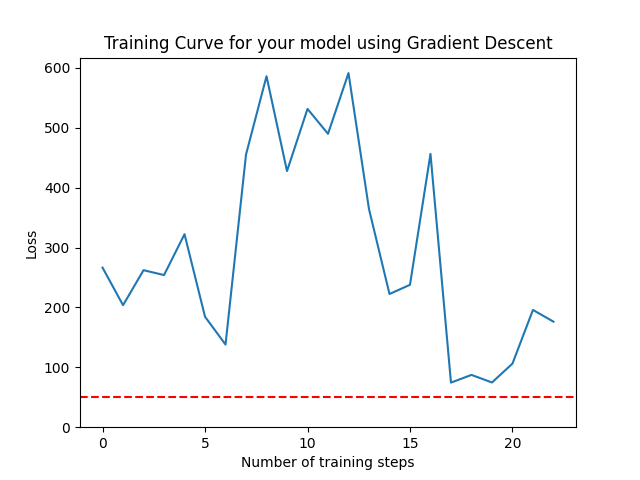
\includegraphics[width=0.4\textwidth]{Figs/Example training.png}
    \caption{ Example caption}
    \label{fig:net}
\end{figure}


\end{document}